\chapter{Commissioning GOTO}
\label{chap:commissioning}
\chaptoc{}

% ########################################

\newpage
\section{Introduction}
\label{sec:commissioning_intro}
\begin{colsection}

% ~~~~~~~~~~~~~~~~~~~~

\begin{colsection}

WIP

\end{colsection}

% ~~~~~~~~~~~~~~~~~~~~

\end{colsection}

% ########################################

\newpage
\section{Detector characterisation}
\label{sec:detectors}
\begin{colsection}

% ~~~~~~~~~~~~~~~~~~~~

\begin{colsection}
It was considered important to carry out a good analysis of the GOTO cameras: firstly to ensure they met the specification given by FLI and secondly to independently test the important characteristics that are unique to each detector.


\end{colsection}

% ~~~~~~~~~~~~~~~~~~~~
\newpage
\subsection{The FLI detectors}
\label{sec:FLI}
\begin{colsection}

The KAF-50100 detectors used in the GOTO cameras consists of a $8304 \times 6220$ pixel CCD with $\SI{6}{\micro\metre} \times \SI{6}{\micro\metre}$ square pixels. It has two channels and either two or four outputs. In our case the two-output system is used, and reads out at 8 MHz. The layout of the sensor is shown below in \aref{fig:chip}, adapted from the ON Semi specification sheet.

The primary active region has an area of 8176 $\times$ 6132 pixels. This is the default frame that excludes any of the surrounding test regions.

The full frame of the camera outputs an 8304 $\times$ 6220 array. Surrounding the active area on each edge are 16 active buffer pixels, which are light-sensitive but not considered part of the primary region. Around the edge of the active area is a border of light-shielded dark reference pixels: 29 dark rows at the start, 26 rows at the end and 28 columns on the sides leading each row. These pixels do not respond to light and therefore can be used as a dark reference. At the beginning and end of each row there is also a CTE test column with 4 blank columns either side, as well as a CTE test row at the end of each frame, included for test purposes. Finally there are 10 dummy pixels leading each row, as well as a final pixel used in the readout process. These dummy pixels form an overscan region which can be used to measure and correct for bias signal.

The software allows for a large amount of overscan in either dimension. Overscan pixels in the vertical will appear at the top of the frame, and will appear to have a dark current level picked up as they are transferred down the frame. Horizontal overscan pixels will appear at the end of each channel, i.e.\ running down the centre of the frame, and will only contain values approximating the readout noise.

A sample frame from Camera 2 is shown in \aref{fig:frame}. You can clearly see the extra regions around the frame, with the lower corner expanded in more detail.

\begin{figure}[p]
    \begin{center}
        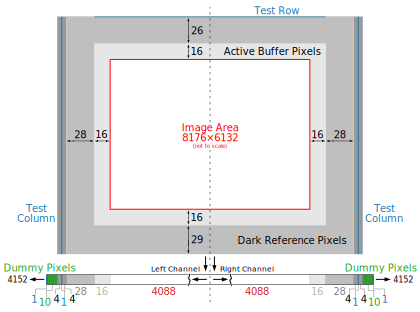
\includegraphics[width=\textwidth]{images/chip}
    \end{center}
    \caption[The layout of the CCD chips in the MicroLine cameras used by GOTO]{
        The layout of the CCD chips in the MicroLine cameras used by GOTO.\@ The central image area is not shown to scale, but the surrounding rows and columns are all in proportion.
        }\label{fig:chip}
\end{figure}

\begin{figure}[p]
    \begin{center}
        \includegraphics[width=\textwidth]{images/sample.png}
    \end{center}
    \caption[TODO]{
        A sample bright frame from one of the GOTO cameras. The highlighted area in the corner shows some of the features described in \aref{fig:chip}. Also note the two bad columns.
        }\label{fig:frame}
\end{figure}

\clearpage

\end{colsection}

% ~~~~~~~~~~~~~~~~~~~~
\subsection{In-lab tests}
\label{sec:detector_tests}
\begin{colsection}

The first of the FLI cameras to be used on GOTO arrived in Warwick in February 2016, and in March it was moved to Sheffield to carry out a detailed study.
The first camera was bought up to Sheffield on 8th March with a collection of other hardware, it was taken back when the other three were delivered on 10th May. These cameras were returned to Warwick on 8th June.

The results of the analysis were written up as a page on the GOTO wiki for easy access and reference, and are repeated below.

% ---------
\newpage
\subsubsection{Defects}

\begin{table}[t]
    \begin{center}
        \begin{tabular}{cc|lll} %chktex 44
            Camera   & Serial    & \multicolumn{3}{c}{Dark Columns} \\
            \midrule
            Camera 1 & ML0010316 & 1 dead column:  & x=7678, starting at y=4312 & (30\%) \\
            Camera 2 & ML0330316 & 2 dead columns: & x=3583, starting at y=909  & (85\%) \\
                     &           &                 & x=6386, starting at y=127  & (98\%) \\
            Camera 3 & ML0420516 & 2 dead columns: & x=1800, starting at y=1151 & (81\%) \\
                     &           &                 & x=5140, starting at y=4986 & (19\%) \\
            Camera 4 & ML0430516 & 1 dead column:  & x=5333, starting at y=2561 & (58\%) \\
        \end{tabular}
    \end{center}
    \caption[TODO]{
        Locations of dead columns caused by stuck pixels. The percentages denote the amount of the column that is unusable.
    }\label{tab:frame}
\end{table}

For each camera a defect mask was constructed using the ratio of two flat images of different exposures, and then detecting pixels outside of a given sigma limit. Each camera was found to have at least one stuck pixel, which produced a dead column travelling up the frame. In \aref{fig:frame} these are visible as two dark columns. The exact positions and details for every camera are shown in \aref{tab:frame}.

The ONSemi chip specifications gives an allowed limit of less than 20 column defects per device, and none of the GOTO detectors had more than two.

% ---------
\newpage
\subsubsection{Bias}

\begin{table}[t]
    \begin{center}
        \begin{tabular}{l l l | c c | c} %chktex 44
            Camera   & Serial    &   & Overscan bias & Field bias  & FLI value \\
                     &           &   & (ADU)         & (ADU)       & (ADU)     \\
            \midrule
            Camera 1 & ML0010316 & L & $\sim 970$    & $ 0 \pm 3$  & $970.6$   \\
                     &           & R & $\sim 960$    & $ 7 \pm 3$  & $965.6$   \\
            Camera 2 & ML0330316 & L & $\sim 985$    & $ 6 \pm 3$  & $995.7$   \\
                     &           & R & $\sim 970$    & $14 \pm 3$  & $988.7$   \\
            Camera 3 & ML0420516 & L & $\sim 990$    & $11 \pm 3$  & $995.9$   \\
                     &           & R & $\sim 975$    & $12 \pm 3$  & $989.0$   \\
            Camera 4 & ML0430516 & L & $\sim 965$    & $10 \pm 3$  & $969.7$   \\
                     &           & R & $\sim 990$    & $11 \pm 4$  & $1000.6$  \\
        \end{tabular}
    \end{center}
    \caption[TODO]{
        Measured bias values for the four cameras. Field bias denotes the remaining bias levels after overscan subtraction.
        }\label{tab:bias}
\end{table}

For a standard full-frame image there are two methods to correct for bias: using the overscan regions and using a master bias.

The two 10-pixel wide dummy regions on either side of the image as shown in \aref{fig:chip} can be subtracted from the frame (independently for each channel) to correct for much of the bias level. These levels change for each image, but typical values for each camera and channel are given in \aref{tab:bias} --- they are usually between 960 and 990 counts.

For each camera 50 dark, zero-exposure full-frame images were taken, overscan subtracted and stacked in order to construct a master bias frame. This can be used to correct for any structure in the bias level. The most obvious structure is a difference in bias levels between the two channels in each camera. The average remaining field bias values are also listed in \aref{tab:bias}.

% ---------
\newpage
\subsubsection{Photon transfer curves}

\begin{table}[p]
    \begin{center}
        \begin{tabular}{lll|cccc|cc} %chktex 44
                     &            &   & \multicolumn{4}{c|}{Sheffield}            & \multicolumn{2}{c}{FLI} \\
                     &            &   & \multicolumn{2}{c}{RON} & Gain     & FPN  & RON       & Gain        \\
                     &            &   & (ADU)      & (e-)       & (e-/ADU) & (\%) & (e-)      & (e-/ADU)    \\
            \midrule
            Camera 1 & 1$\times$1 & L & 23.0       & 12.0       & 0.52     & 0.23 & 12.1      & 0.53        \\
                     &            & R & 22.1       & 11.3       & 0.51     & 0.22 & 11.6      & 0.53        \\
                     & 2$\times$2 & L & 27.5       & 14.3       & 0.52     & 0.17 & ---       & ---         \\
                     &            & R & 26.5       & 13.5       & 0.52     & 0.16 & ---       & ---         \\
                     & 3$\times$3 & L & 32.6       & 16.9       & 0.53     & 0.16 & ---       & ---         \\
                     &            & R & 31.2       & 15.9       & 0.52     & 0.14 & ---       & ---         \\
            \midrule
            Camera 2 & 1$\times$1 & L & 22.3       & 11.8       & 0.54     & 0.26 & 11.8      & 0.54        \\
                     &            & R & 22.1       & 11.7       & 0.54     & 0.28 & 11.9      & 0.55        \\
                     & 2$\times$2 & L & 27.1       & 14.4       & 0.52     & 0.15 & ---       & ---         \\
                     &            & R & 25.9       & 13.7       & 0.54     & 0.17 & ---       & ---         \\
                     & 3$\times$3 & L & 31.8       & 16.9       & 0.53     & 0.12 & ---       & ---         \\
                     &            & R & 30.2       & 16.0       & 0.53     & 0.14 & ---       & ---         \\
            \midrule
            Camera 3 & 1$\times$1 & L & 22.1       & 12.8       & 0.60     & 0.28 & 12.9      & 0.59        \\
                     &            & R & 20.7       & 12.0       & 0.58     & 0.24 & 12.2      & 0.59        \\
                     & 2$\times$2 & L & 25.5       & 14.8       & 0.58     & 0.17 & ---       & ---         \\
                     &            & R & 24.3       & 14.1       & 0.57     & 0.15 & ---       & ---         \\
                     & 3$\times$3 & L & 29.6       & 17.2       & 0.60     & 0.16 & ---       & ---         \\
                     &            & R & 28.5       & 16.5       & 0.58     & 0.12 & ---       & ---         \\
            \midrule
            Camera 4 & 1$\times$1 & L & 23.0       & 13.6       & 0.59     & 0.26 & 14.1      & 0.60        \\
                     &            & R & 23.4       & 13.8       & 0.59     & 0.25 & 14.0      & 0.59        \\
                     & 2$\times$2 & L & 26.7       & 15.8       & 0.60     & 0.18 & ---       & ---         \\
                     &            & R & 27.2       & 16.1       & 0.60     & 0.16 & ---       & ---         \\
                     & 3$\times$3 & L & 30.6       & 18.1       & 0.60     & 0.17 & ---       & ---         \\
                     &            & R & 31.6       & 18.6       & 0.60     & 0.15 & ---       & ---         \\
        \end{tabular}
    \end{center}
    \caption[TODO]{
        Results of fitting photon transfer curves for each of the four cameras, at three different binning factors. The values on the right come from FLI's individual spec sheets for each camera. Directly comparable values are highlighted.
        }\label{tab:ptc}
\end{table}

Photon transfer curves were constructed for each camera for 1$\times$1, 2$\times$2 and 3$\times$3 binning factors. The results are shown in \aref{tab:ptc} below, with values for the readout noise, gain and fixed-pattern (flat field) noise found by fitting to the theoretical curve. These can also be compared to the values measured by FLI, which were only recorded for 1$\times$1 binning factor. Three PTCs for Camera 1 are shown in \aref{fig:ptc}.

\begin{figure}
    \begin{center}
        \includegraphics[width=0.87\textwidth]{images/1comb.pdf}
    \end{center}
    \caption[TODO]{
        The three constructed photon transfer curves for Camera 1. In general the read-out noise increases with on-chip binning, while the fixed-pattern noise decreases.
        }\label{fig:ptc}
\end{figure}

% ---------
\newpage
\subsubsection{Linearity}
Linearity was measured for all four cameras using a flat light source and increasing exposure times. Each camera had a turn off in the lower half of the dynamic range which needs further analysis, this experiment was hampered by the broken flat light source. Very short exposure times were studied in order to see any possible effect of the shutter speed. It was found that although the cameras allow exposure times as low as 1ms there is a consistent deviation from linearity below approximately 0.15 seconds. As such exposure times shorter than 0.2 seconds should be avoided.

% ---------
\newpage
\subsubsection{Dark current}

\begin{table}
    \begin{center}
        \begin{tabular}{ll|cc} %chktex 44
            Camera   & Serial    & Dark current @ -25degree C & DC doubling temp. \\
                     &           & (e-/pix/sec)               & (degree C)        \\
            \midrule
            Camera 1 & ML0010316 & $0.0020$                   & $10.8$            \\
            Camera 2 & ML0330316 & $0.0018$                   & $9.8$             \\
            Camera 3 & ML0420516 & $0.0022$                   & $10.9$            \\
            Camera 4 & ML0430516 & $0.0015$                   & $9.0$             \\
        \end{tabular}
    \end{center}
    \caption[TODO]{
        Measured dark current values for the four cameras. The initial FLI spec was for $0.002$~electrons/pixel/second, but this was later revised up to $0.008$ e-/pix/sec.
        }\label{tab:dark}
\end{table}

Dark current was analysed as a function of temperature. This required long (30 minute) dark exposures, taken overnight to reduce background light. Each camera produced a clear exponential trend, a curve was fitted defined by the dark current at -25°C (an arbitrary point, but matched to the spec definition) and the dark current doubling temperature. The results are shown in \aref{tab:dark}.

The preliminary specification sheet gave a typical value of 0.002 electrons/pixel/second for the dark current at -25°C, all the cameras were around this value although with some deviation. The revised spec gave an expected value of 0.008 e-/pix/sec, well above what we measure.

The dark current was also examined as a function of time since power on, as in some cameras (such as ULTRASPEC) the dark current reduces slowly. No such trend was visible using the FLI cameras. However since the detector and cooler are integrated into the same body there has to be some time spent waiting after power on for the camera to cool to the target temperature, thus negating the effect.

% ---------
\newpage
\subsubsection{Timing}
An analysis was carried out attempting to measure the readout speeds of the CCD, and thus the minimum dead time required for a given frame. However, as the cameras do not have enough memory to store an entire frame (communication with FLI) readout must begin immediately after the exposure has finished in order to prevent the data being overwritten. This typically takes approximately 3 seconds for a full frame.

% ---------
\newpage
\subsubsection{Results}

Overall the initial characterization of the detectors managed to agree with the specifications provided by FLI.\@ In the case of the critical PTC values (gain, noise etc\ldots) FLI carried out their own analysis which I only received the results of after my own analysis had finished. These are given in \aref{tab:ptc} and show very similar results to the ones observed in Sheffield. More complete characterization will be possible once the telescope is up an running, in particular using the sky for flat-field and point-source tests which were limited by the equipment available here.

\end{colsection}

% ~~~~~~~~~~~~~~~~~~~~
\newpage
\subsection{Throughput modelling}
\label{sec:throughput}
\begin{colsection}

WIP

\end{colsection}

% ~~~~~~~~~~~~~~~~~~~~

\end{colsection}

% ########################################

\newpage
\section{Deploying the hardware}
\label{sec:hardware}
\begin{colsection}

% ~~~~~~~~~~~~~~~~~~~~

\begin{colsection}

WIP

\end{colsection}

% ~~~~~~~~~~~~~~~~~~~~

\subsection{Construction on La Palma}
\label{sec:construction}
\begin{colsection}

WIP

\end{colsection}

% ~~~~~~~~~~~~~~~~~~~~

\subsection{Extra dome systems}
\label{sec:arduino}
\begin{colsection}

WIP

\end{colsection}

% ~~~~~~~~~~~~~~~~~~~~

\end{colsection}

% ########################################

\newpage
\section{Developing observing routines}
\label{sec:obs_scripts}
\begin{colsection}

% ~~~~~~~~~~~~~~~~~~~~

\begin{colsection}

WIP

\end{colsection}

% ~~~~~~~~~~~~~~~~~~~~

\subsection{Taking flat fields}
\label{sec:flats}
\begin{colsection}

WIP \citep{flats}

\end{colsection}

% ~~~~~~~~~~~~~~~~~~~~

\subsection{Focusing the telescopes}
\label{sec:autofocus}
\begin{colsection}

WIP \citep{autofocus}

\end{colsection}

% ~~~~~~~~~~~~~~~~~~~~

\end{colsection}

% ########################################

\newpage
\section{Observing results}
\label{sec:observing}
\begin{colsection}

% ~~~~~~~~~~~~~~~~~~~~

\begin{colsection}

WIP

\end{colsection}

% ~~~~~~~~~~~~~~~~~~~~

\subsection{The all-sky survey}
\label{sec:survey_results}
\begin{colsection}

WIP

\end{colsection}

% ~~~~~~~~~~~~~~~~~~~~

\subsection{Gravitational wave observations}
\label{sec:gw_results}
\begin{colsection}

WIP

\end{colsection}

% ~~~~~~~~~~~~~~~~~~~~

\subsection{Other transient follow-up}
\label{sec:other_results}
\begin{colsection}

WIP

\end{colsection}

% ~~~~~~~~~~~~~~~~~~~~

\end{colsection}

% ########################################
